%%%%%%%%%%%%%%%%%%%%%%%%%%%%%%%%%%%%%%%%%%%%%%%%%%%%%%%%%%%%%%%%%%%%%%%%%%%%%%%%%%%
% MODEL MADE BY PRUNELLE DAUDRÉ--TREUIL, USE AT YOUR OWN RISK, YOU HAVE BEEN      %
% WARNED !                                                                        %
% COPYRIGHT : CC-BY-SA                                                            %
% LAST UPDATE : 12-04-2024                                                        %
%%%%%%%%%%%%%%%%%%%%%%%%%%%%%%%%%%%%%%%%%%%%%%%%%%%%%%%%%%%%%%%%%%%%%%%%%%%%%%%%%%%

%%%%%%%%%%%%%%%%%%%%%%%%%%%%%%%%%%%%%%%%%%%%%%%%%%%%%%%% Compilation option
\documentclass{beamer} % the most basic compilation

%\documentclass[draft]{beamer} % to compile quickly without image
%\documentclass[handout]{beamer} % to compile whithout transitions (handout) + following lines
%\usepackage{pgfpages}
%\pgfpagesuselayout{2 on 1}[a4paper,border shrink=5mm] % 2 slides by page, vertical
%\pgfpagesuselayout{4 on 1}[a4paper,landscape,border shrink=5mm] % 4 slides by page, horizontal
%\pgfpagesuselayout{8 on 1}[a4paper,border shrink=5mm] % 8 slides by page, vertical
%\pgfpagesuselayout{16 on 1}[a4paper,landscape,border shrink=5mm] % 16 slides by page, horizontal 
%\documentclass{article} % tansform the slides in article, attention a lot of lines that change
%\usepackage{beamerarticle} % parameters will react strangely to it

%%%%%%%%%%%%%%%%%%%%%%%%%%%%%%%%%%%%%%%%%%%%%%%%%%%%%%%% Configuration

% THE ORDER IS IMPORTANT PRETTY PLEASE

%%%%%%%%%%%%%%%%%%%%%%%%%%%%%%%%%%%%%%%%%%%%%%%%%%%%%%%% Packages
\usepackage{graphicx} % Required for inserting images
\usepackage{amsmath}
\usepackage{hyperref}
\usepackage{animate}
\usepackage[framemethod=TikZ]{mdframed}
\usepackage{appendixnumberbeamer}
\usepackage[backend=bibtex,style=authoryear,natbib=true]{biblatex} % Add/delete lib here
%%%%%%%%%%%%%%%%%%%%%%%%%%%%%%%%%%%%%%%%%%%%%%%%%%%%%%%% Personal informations
\title{INTERNSHIIIIIP}
\subtitle{A pretty subtitle}
\author{Prunelle Daudré--Treuil}
\date{\today}
\institute{Msc TAL 22-24\\Université de Lorraine}
\def\supervisor{Mr. RANDOM}
\def\company{LORIA ?}

%%%%%%%%%%%%%%%%%%%%%%%%%%%%%%%%%%%%%%%%%%%%%%%%%%%%%%%% Import
\def\logo{img/logos/pretty.png}
\def\logoSection{img/logos/pretty.png}
\def\logoCompany{img/logos/loria.png}

\bibliography{sample} % Put your information here
%%%%%%%%%%%%%%%%%%%%%%%%%%%%%%%%%%%%%%%%%%%%%%%%%%%%%%%% Color Palette
% I'm just trying to find a color palette for université de lorraine <3
\definecolor{main}{rgb}{0.74, 0.2, 0.64}
\definecolor{light}{rgb}{1.00,0.90,0.98}
\definecolor{arylideyellow}{rgb}{0.91, 0.84, 0.42}
\definecolor{bananamania}{rgb}{0.98, 0.91, 0.71}

%%%%%%%%%%%%%%%%%%%%%%%%%%%%%%%%%%%%%%%%%%%%%%%%%%%%%%%% Metropolis theme
\usetheme[numbering=fraction, progressbar=frametitle]{metropolis}
\usecolortheme{seahorse}
\setbeamercolor*{palette primary}{use=structure,fg=black,bg=arylideyellow}
%\setbeamercovered{transparent} 
\setbeamertemplate{background canvas}[vertical shading][bottom=lightgray!10,top=arylideyellow!20]
\setbeamerfont{section in toc}{size=\Large}

%%%%%%%%%%%%%%%%%%%%%%%%%%%%%%%%%%%%%%%%%%%%%%%%%%%%%%%% Progression bar
\makeatletter
\setlength{\metropolis@titleseparator@linewidth}{2pt}
\setlength{\metropolis@progressonsectionpage@linewidth}{2pt}
\setlength{\metropolis@progressinheadfoot@linewidth}{2pt}
\makeatother

%%%%%%%%%%%%%%%%%%%%%%%%%%%%%%%%%%%%%%%%%%%%%%%%%%%%%%%% Pretty Box
\global\mdfdefinestyle{box}{%
middlelinewidth=2pt, linecolor=arylideyellow,roundcorner=5pt, backgroundcolor=bananamania
}

%%%%%%%%%%%%%%%%%%%%%%%%%%%%%%%%%%%%%%%%%%%%%%%%%%%%%%%% Table of content
\newcommand{\maketoc}{
    \label{toc}
    %\setbeamertemplate{section in toc}[circle]
    %\tableofcontents[hideallsubsections]
    \part{Table of contents}}

%%%%%%%%%%%%%%%%%%%%%%%%%%%%%%%%%%%%%%%%%%%%%%%%%%%%%%%% Random DON'T TOUCH
\pdfstringdefDisableCommands{%
\def\translate#1{#1}%
} % Must not touch if not a LaTeX expert
%%%%%%%%%%%%%%%%%%%%%%%%%%%%%%%%%%%%%%%%%%%%%%%%%%%%%%%% Title page (don't modify)

\setbeamertemplate{title page}{
    \begin{minipage}[c][\paperheight]{\textwidth}
        \ifx\inserttitlegraphic\@empty\else\usebeamertemplate*{title graphic}\fi
        \vfill
        \ifx\inserttitle\@empty\else\usebeamertemplate*{title}\fi
        \ifx\insertsubtitle\@empty\else\usebeamertemplate*{subtitle}\fi
        \usebeamertemplate*{title separator}
        \begin{minipage}[t]{.5\textwidth}
            \ifx\beamer@shortauthor\@empty\else\usebeamertemplate*{author}\fi
            \vspace*{0.5em}
            \ifx\insertdate\@empty\else\usebeamertemplate*{date}\fi
            \ifx\insertinstitute\@empty\else\usebeamertemplate*{institute}\fi
        \end{minipage}
        \begin{minipage}[t]{.5\textwidth}
            \vspace*{2em}
            {\hspace{3.2em}\small Supervisor: \textit{supervisor} \par}
            \vspace*{0.2em}
            {\hspace{3.2em}\small Company: \textit{\company}}
        \end{minipage}
        \vfill
        \hspace{9.7cm}\scalebox{.4}{Beamer model by Prunelle DT}
    \end{minipage}
}

%%%%%%%%%%%%%%%%%%%%%%%%%%%%%%%%%%%%%%%%%%%%%%%%%%%%%%%% Titlegraphic (can modify)
% Attention, you will go crazy trying to place your image, if you don't see some, you push them outside of the frame, try reducing your vspace/hspace to see it again, good luck <3
% Notes for all images : prefer transparant background to white one, crop them precisely to be able to place them where you want withouh overfull hbox/vbox
\titlegraphic{ 
    {\hspace{8.2cm}\includegraphics[height=3cm]{\logo}}
    
    \vspace{3.6cm}
    
    {
\includegraphics[width=2.5cm]{config/logos/idmc.png}
    \hspace{0.5cm}
    
\includegraphics[width=2cm]{config/logos/ul.png}
    \hspace{2.2cm}
    \includegraphics[width=3cm]{\logoCompany}
}}

%%%%%%%%%%%%%%%%%%%%%%%%%%%%%%%%%%%%%%%%%%%%%%%%%%%%%%%% Section page
\AtBeginSection{
  \frame[plain,noframenumbering]{
    \sectionpage
    \center\hyperlink{toc}{\includegraphics[height=4cm]{\logo}}
}}

%%%%%%%%%%%%%%%%%%%%%%%%%%%%%%%%%%%%%%%%%%%%%%%%%%%%%%%% Subsection page
\AtBeginSubsection{
  \frame[plain,noframenumbering]{
    \subsectionpage
    \center\hyperlink{toc}{\includegraphics[height=4cm]{\logo}}
  }}

%%%%%%%%%%%%%%%%%%%%%%%%%%%%%%%%%%%%%%%%%%%%%%%%%%%%%%%% Part page (appendice)
\setbeamertemplate{part page}{
        \begin{beamercolorbox}[sep=8pt,center,wd=\textwidth]{part title}
            \usebeamerfont{part title}\insertpart\par
        \end{beamercolorbox}
}

\makeatletter
\AtBeginPart{%
  \beamer@tocsectionnumber=0\relax
  \setcounter{section}{0}
  \frame[plain,noframenumbering]{
    \partpage
    \setbeamertemplate{section in toc}[circle]
    \tableofcontents[hideallsubsections]
  }
}
\makeatother
 % Section page easy to change, title graphic is a challenge
\usepackage{tikz}

%%%%%%%%%%%%%%%%%%%%%%%%%%%%%%%%%%%%%%%%%%%%%%%%%%%%%%%% TiKz libraries

\usetikzlibrary{spy} % for "zooming in" pictures
\usetikzlibrary {arrows.meta}
\usetikzlibrary {positioning}
\usetikzlibrary {shapes.geometric}
\usetikzlibrary {decorations.pathmorphing}

%%%%%%%%%%%%%%%%%%%%%%%%%%%%%%%%%%%%%%%%%%%%%%%%%%%%%%%% TiKz style

\tikzstyle{individual}=[rectangle,draw=orange!50,fill=orange!20,thick]
\tikzstyle{concept}=[rectangle,draw=blue!50,fill=blue!20,thick]
\tikzstyle{litteral}=[rectangle,text=red]
\tikzstyle{pre}=[<-,>={Stealth[round]},semithick]
\tikzstyle{post}=[->,>={Stealth[round]},semithick] % To configure tikz if needed



%%%%%%%%%%%%%%%%%%%%%%%%%%%%%%%%%%%%%%%%%%%%%%%%%%%%%%%% DOCUMENT BODY   

\begin{document}

\maketitle
\maketoc
%\label{toc}
%\part{Table of contents}
%%%%%%%%%%%%%%%%%%%%%%%%%%%%%%%%%%%%%%%%%%%%%%%%%%%%%%%% Examples slides
\section{Introduction}

\begin{frame}{Analogy in CBR}

    \centering\emph{"Every time I forgot my umbrella, it is raining, so if I forgot my umbrella it will rain"}

    \vspace{0.85cm}

    \begin{mdframed}[style=box] 

    A little bit of text
     \end{mdframed}

    \vspace{0.85cm}

    \centering\textbf{Similar situations have similar outcomes}

\end{frame}

%%%%%%%%%%%%%%%%%%%%%%%%%%%%%%%%%%%%%%%%%%%%%%%%%%%%%%%%

\begin{frame}{The CoAT method}
    
    \vspace{0.25cm}

    \begin{mdframed}[style=box] % A simpler example of yellow boxes
         \textbf{Ordinal constraint :} \emph{If $S_0$ is more similar to $S_i$ than to $S_j$ then the same thing should be true for the outcomes}
     \end{mdframed}
    
    \vspace{0.25cm}
    
    \begin{center}
        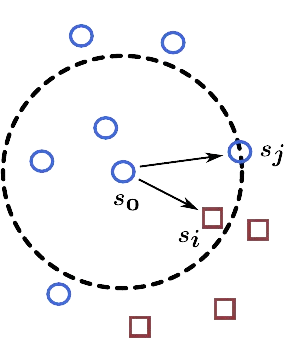
\includegraphics[scale=0.25]{img/logos/pretty.png}
    \end{center}
    
    \vspace{0.25cm}

    \begin{mdframed}[style=box]
         \textbf{The CoAT indicator :} $\Gamma (CB, \sigma_S, \sigma_R)$ = number of triples \\$(S_0, S_i, S_j)$ where the constraint is not respected
     \end{mdframed}
    
\end{frame}

%%%%%%%%%%%%%%%%%%%%%%%%%%%%%%%%%%%%%%%%%%%%%%%%%%%%%%%%

\begin{frame}<1>[label=dist]{Distance} % you will see what dark magic i will do with that label

    \vspace{0.5cm} % some math examples
    
    \textbf{Euclidean Distance:} $$d_E = \sqrt{(x_1 - x_2)^2+(y_1 - y_2)^2}$$

    \textbf{Manhattan Distance:} $$ d_{Man} = |x_1-x_2|+|y_1-y_2|$$

    \textbf{The Minkoswki Distance:} $$d_{Mk}^p =  [(x_1-x_2)^p + (y_1-y_2)^p]^{\frac{1}{p}} $$

    \textbf{Mahalanobis Distance:} $$D_{\text{mahal}}= \sqrt{(x-y)^T M^{-1} (x-y)}$$
    
\end{frame}

%%%%%%%%%%%%%%%%%%%%%%%%%%%%%%%%%%%%%%%%%%%%%%%%%%%%%%%%

\section{Regression}
\subsection{With Generated Data}

\begin{frame}{With Generated Data (1)}
    Generating Function : $2 \times x + 1$
    
    Noise function : \textit{Gaussian distribution with $\sigma$ = 100 and $\mu$ = 0}
    \begin{figure}
        \centering
        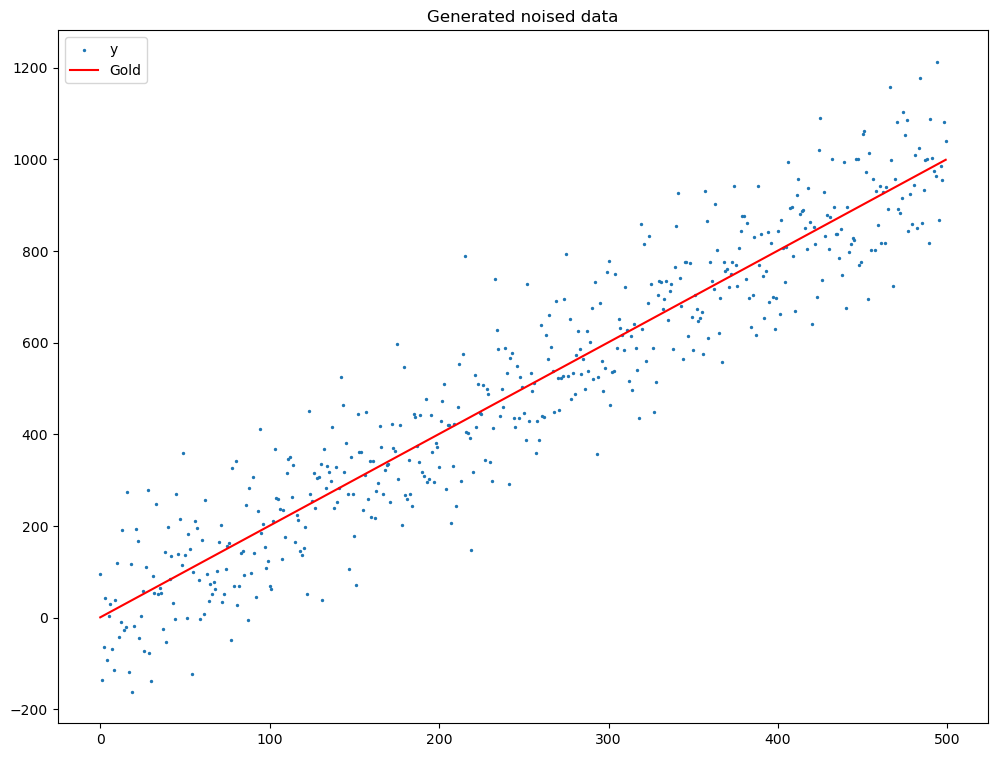
\includegraphics[scale=0.35]{img/a.png}
    \end{figure}
\end{frame}

%%%%%%%%%%%%%%%%%%%%%%%%%%%%%%%%%%%%%%%%%%%%%%%%%%%%%%%%

\begin{frame}<1>[label=zooms]{With Generated Data (2)}

    \framezoom<1><2>(0cm,0cm)(4cm,3.7cm) % we specify where to zoom (coordinate of the top-left 
    \framezoom<1><3>(6cm,0cm)(4cm,3.7cm) % angle of the rectangle)(size rectangle)
	
    \begin{columns} % A better way to have 2 columns than minipage, doesn't work in the yellow boxes
        \begin{column}{0.48\textwidth}
            \begin{figure}
                \centering
                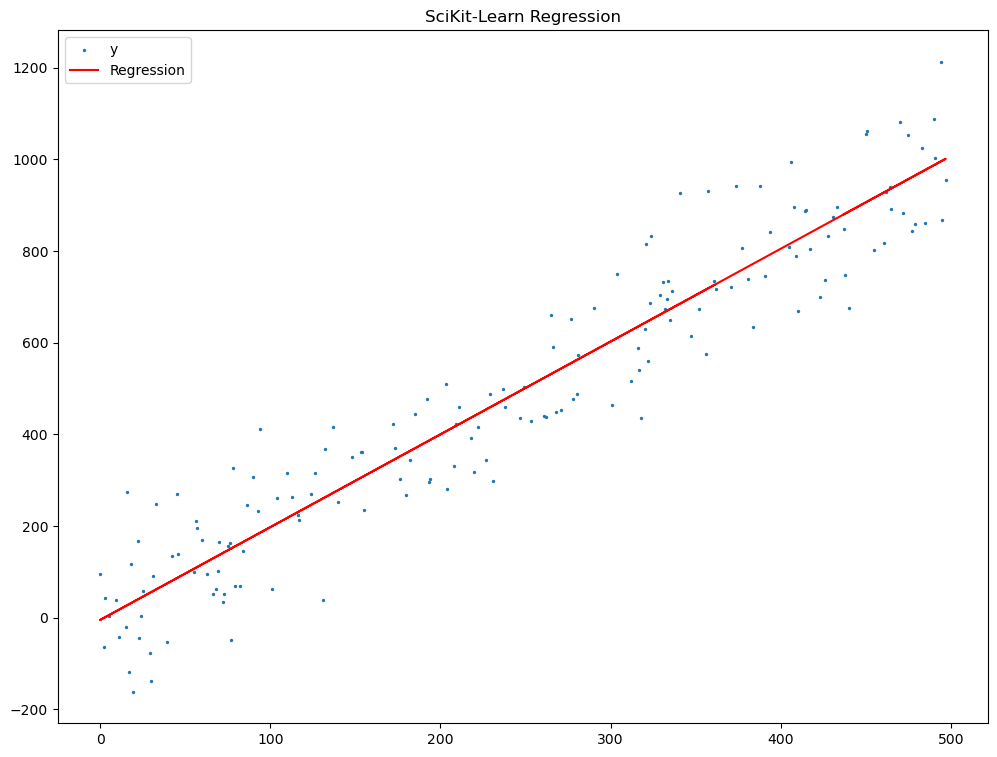
\includegraphics[width=0.9\textwidth]{img/b.png}
                Regression with SciKit-learn
            \end{figure}
        \end{column}
        \begin{column}{0.48\textwidth}
            \begin{figure}
                \centering
                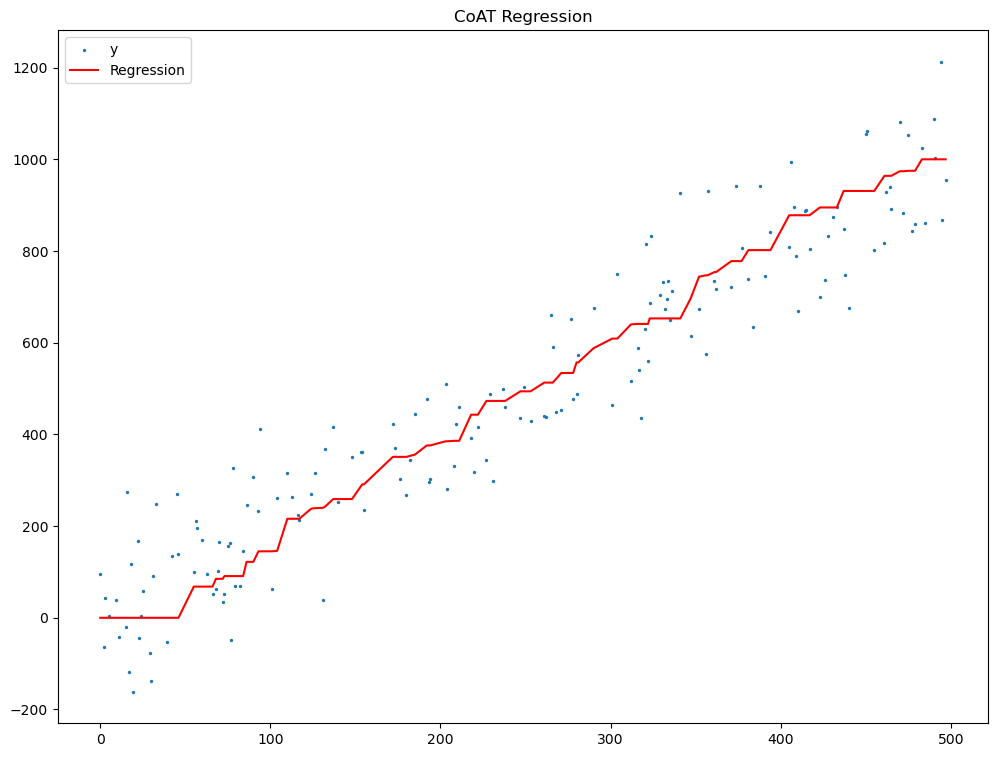
\includegraphics[width=0.9\textwidth]{img/c.png}
                Regression with CoAT
            \end{figure}
        \end{column}
    \end{columns}

    \vspace{0.3cm}

    \begin{mdframed}[style=box]
    \begin{itemize}
        \item Impact of different source and outcomes similarities
        \item Comparison with NN for benchmarking
        \item Real Datasets (multidimensions)
    \end{itemize}
     \end{mdframed}
    
\end{frame}

\againframe<2->[plain]{zooms} % to have it without title

%%%%%%%%%%%%%%%%%%%%%%%%%%%%%%%%%%%%%%%%%%%%%%%%%%%%%%%%

\againframe<2>{dist} % dark magic, i put an old frame again

%%%%%%%%%%%%%%%%%%%%%%%%%%%%%%%%%%%%%%%%%%%%%%%%%%%%%%%%

\begin{frame}{Where do we live ?}

    \begin{tikzpicture}[
    spy using outlines={
      circle,
      magnification=10,
      size=5cm,
      connect spies}]
    \node[inner sep=0pt] {\pgfimage[width=0.4\textwidth]{img/map.jpg}};
    \only<2>{\spy[red!70!black] on (1.2,0.8) in node at (.5\textwidth,0);}
    \end{tikzpicture} % on (0,0) -> center of the picture, (pos, pos) -> top-right corner
    % (neg, neg) -> bottom-left corner
    \only<3>{
        \raisebox{9ex}{
            \begin{minipage}{0.5\textwidth} % The raisebox in minipage technique again
            \centering \Large Elle est pas belle ma France ?
            \end{minipage}
        }}
    
\end{frame}

%%%%%%%%%%%%%%%%%%%%%%%%%%%%%%%%%%%%%%%%%%%%%%%%%%%%%%%%

\subsection{Problems}

\begin{frame}{The problem(s) with regression}
    \textbf{Why I have lost my mind:} A prediction issue

    \begin{itemize}
        \item 10+mn for 165 cases
        \vspace{0.2cm}
        \item Prediction item by item vs prediction by list
        \vspace{0.2cm}
        \item A problem with $y\_values$ ?
        \begin{itemize}
            \item \textit{range(function(500))}
            \item \textit{range(0,function(500),10)}
            \item \textit{range(0,function(500),100)}
        \end{itemize}
        \vspace{0.2cm}
        \item A problem with the number of case ?


    \end{itemize}
    
\end{frame}

% \section{An efficiency metric}

\begin{frame}{A new metric (1)}

    \begin{mdframed}[style=box]
        $$Eff(m,t,p) = \exp^{-\log \left( \dfrac{m}{p+t}\right)}, \;\text{where}$$
    \end{mdframed}

    \vspace{0.5cm}
    
    $p \rightarrow \text{number of parameters in the model},$
    $t \rightarrow \text{time for running the algorithm/model}$
    $m \rightarrow \text{any known metric like F-1, mse etc.}$
    
    \vspace{0.5cm}
    
    \textbf{Note: }The metric should be adapted in function of the known original metric
    
\end{frame}

%%%%%%%%%%%%%%%%%%%%%%%%%%%%%%%%%%%%%%%%%%%%%%%%%%%%%%%%

\begin{frame}{A new metric (2)}
    
    \vspace{0.2cm}

    \begin{mdframed}[style=box]
        $$Eff(m,t,p) = \exp^{-\log \left( \dfrac{m}{p+t}\right)}, \;\text{where}$$
    \end{mdframed}
    
    \vspace{0.2cm}

    \begin{columns} % Another exemple of presentation in two columns
        \begin{column}{0.5\textwidth}
            \center
            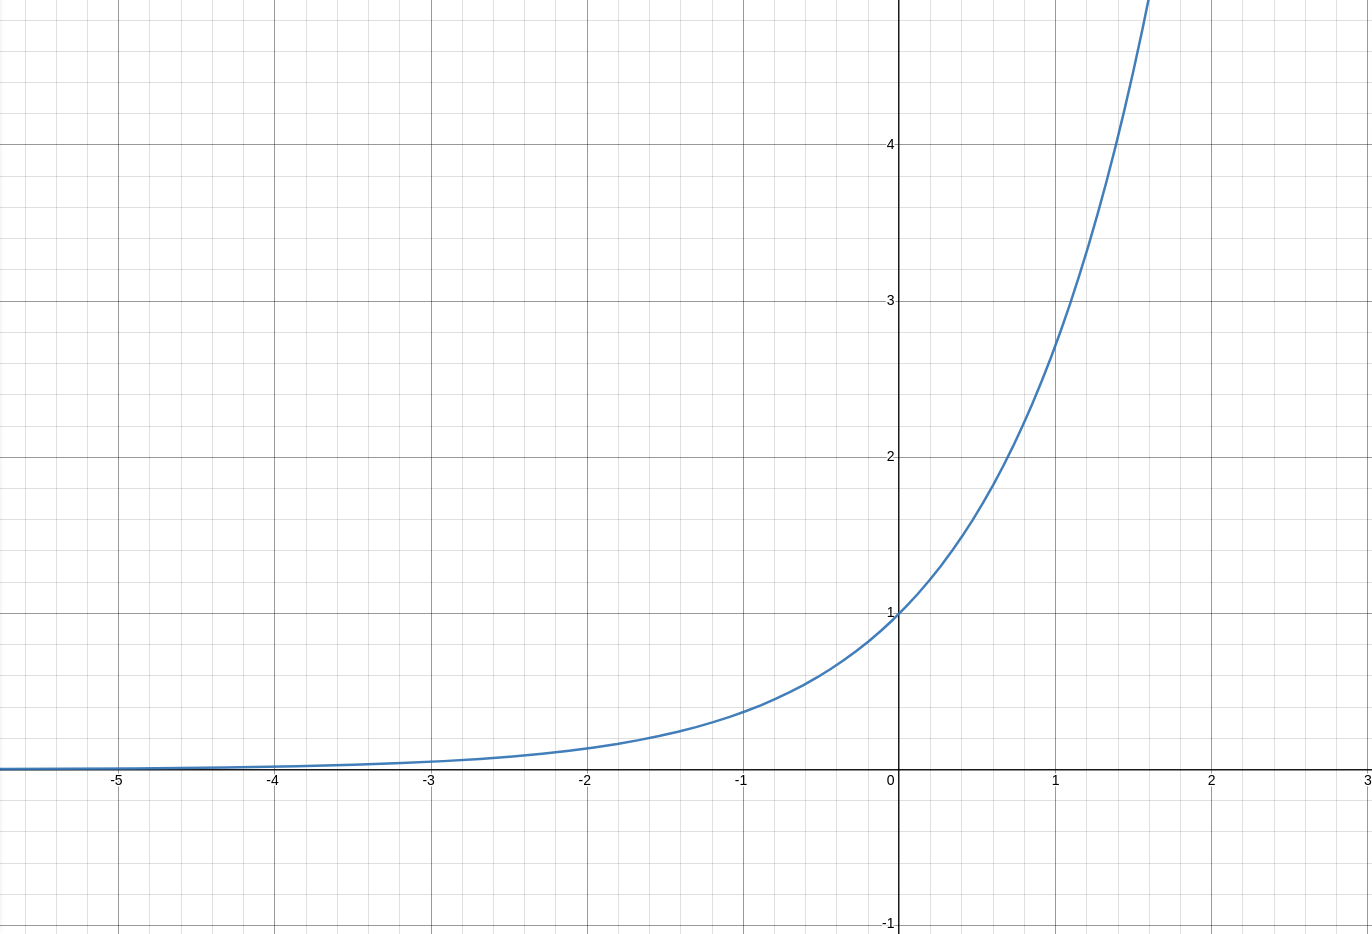
\includegraphics[scale=0.075]{img/exp.png}

            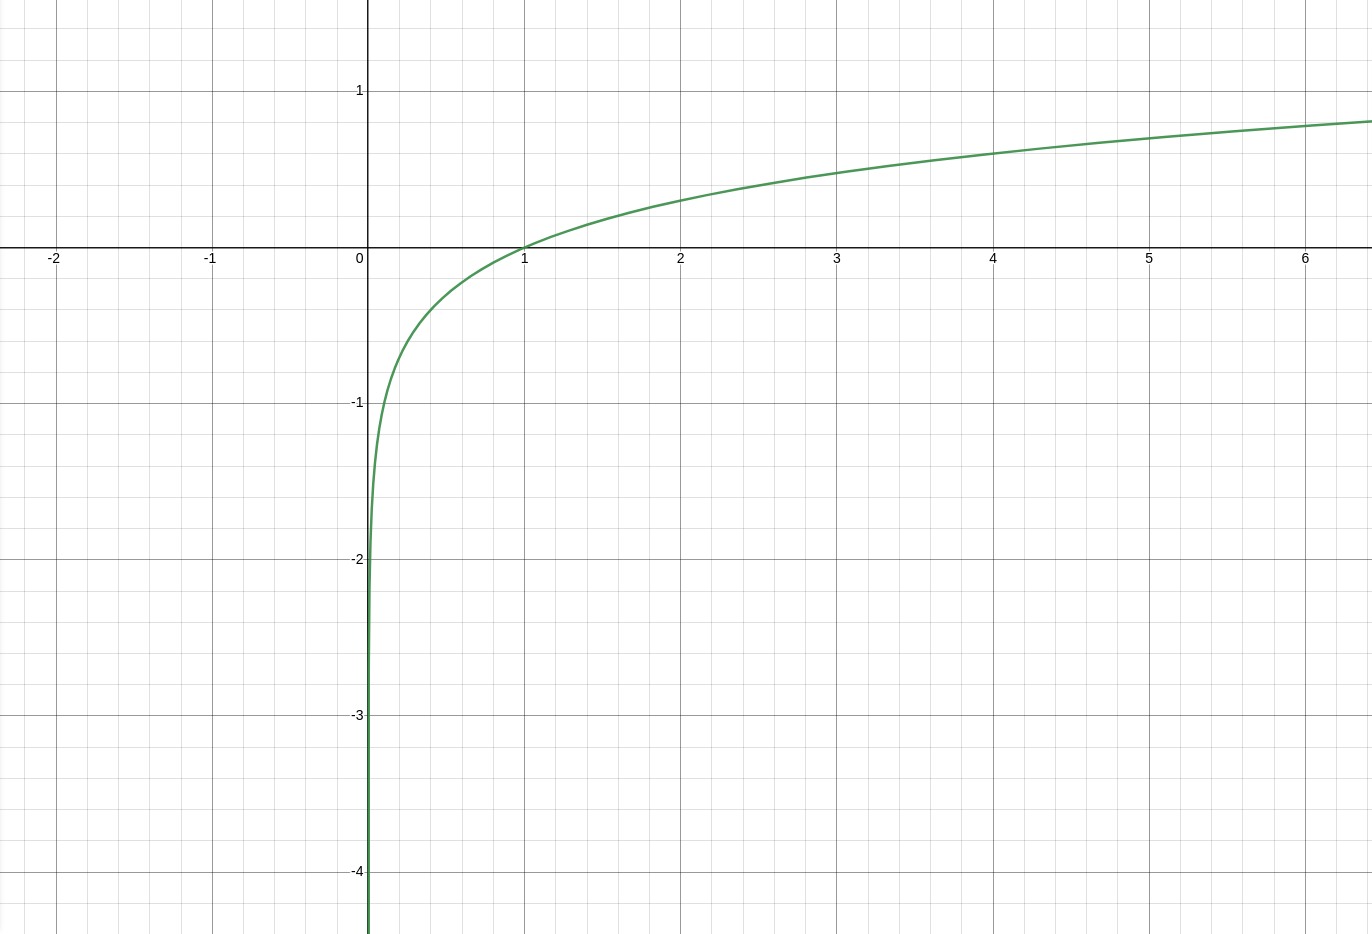
\includegraphics[scale = 0.075]{img/log.png}
        \end{column}
        \begin{column}{0.5\textwidth}
            \vspace{-1cm}
            \center
            $$p \to \infty \Rightarrow \text{metric}_{\text{new}} \to \infty$$
            $$t \to \infty \Rightarrow \text{metric}_{\text{new}} \to \infty$$
            $$m \to \infty \Rightarrow \text{metric}_{\text{new}} \to 0$$
        \end{column}
    \end{columns}
    
\end{frame}
% \section{Some cool tricks}
\subsection{Overlays}

\begin{frame}{The most simple example}

    \small \centering Freedom was a livestream concert by Filipino singer Regine Velasquez (pictured) held on February 28, 2021.\pause Following the cancellation of music events during the outbreak of the COVID-19 pandemic, Velasquez organized the show to create a live experience on a stream for her fans longing for a sense of human connection.\pause The concert's premise was "freedom of singing", stemming from her desire to cover songs from several music genres.\pause It was filmed at the studios of ABS-CBN in Metro Manila, with musicians, background vocalists, and dancers on set, and was broadcast through four livestreaming platforms worldwide.\pause Its set featured a large LED screen as a backdrop and props resembling origami cranes hanging from the ceiling.\pause She performed numerous selections from artists such as Elton John, Chris Isaak, George Michael, Sara Bareilles, Dua Lipa, and Billie Eilish.\pause Critics gave the show high praise for its production and vocal performances, setting a benchmark for online concerts in the Philippines.
    
\end{frame}

%%%%%%%%%%%%%%%%%%%%%%%%%%%%%%%%%%%%%%%%%%%%%%%%%%%%%%%%

\begin{frame}{How Much Can I Put On a Frame?}

    \begin{enumerate}
        \item<1->  A usual frame should have between 20 and 40 words. The maximum should be at about 80 words
        \item<2->  Do not assume that everyone in the audience is an expert on the subject matter, give definition
        \item<3->  Never put anything on a slide that you are not going to explain during the talk
        \item<4->  Keep it simple. Typically, your audience will see a slide for less than 50 seconds
        \item<5->  Less math is better, use English
    \end{enumerate}
    
\end{frame}

%%%%%%%%%%%%%%%%%%%%%%%%%%%%%%%%%%%%%%%%%%%%%%%%%%%%%%%%

\begin{frame}{Structuring a Frame}

    \begin{enumerate} % + -> increment without giving a number everytime
        \item<+-| alert@+> Use block environments
        \item<+-| alert@+> Prefer enumerations and itemize environments
        \item<+-| alert@+> Do not itemize in itemize (same with enumerate)
        \item<+-| alert@+> Do not create endless itemize or enumerate lists
        \item<+-| alert@+> Do not uncover lists piecewise ( what i'm currently doing)
        \item<+-| alert@+> Emphasis is an important part of creating structure
        \item<+-| alert@+> Use columns
        \item<+-| alert@+> Never use footnotes
        \item<+-| alert@+> Use quote or quotation to typeset quoted text
        \item<+-| alert@+> Do not use the option allowframebreaks except for long bibliographies
        \item<+-| alert@+> Do not use long bibliographies
    \end{enumerate}
    
\end{frame}

%%%%%%%%%%%%%%%%%%%%%%%%%%%%%%%%%%%%%%%%%%%%%%%%%%%%%%%%

\begin{frame}{Writing the Text}

    \uncover<1-2>{\centering \large USE SHORT SENTENCES} % the rest of the slide doesn't move when this disappear

    \begin{enumerate}
        \item<1-> Prefer phrases over complete sentences % <1-> means from slide 1 to the end
        \item<1-> Punctuate correctly: no punctuation after phrases, complete punctuation in and after complete sentences % <1-2> for slides 1 and 2
        \item<2-> Never use a smaller font size to “fit more on a frame.” Never ever use the evil option shrink % here we have 2 point appaering in thesame time
        \item<2-> Do not hyphenate words 
        \item<2-2> Break lines “by hand” using the command \textbackslash\textbackslash . Do not rely on automatic line breaking
        \item<1-2> Do not hyphenate words 
    \end{enumerate}

    \uncover<3->{Don't wrote \textit{too much}.} % then later this appear
    
\end{frame}

\begin{frame}[fragile]{An Algorithm For Finding Prime Numbers.} % use fragile for verbatim or lstlisting
    \begin{verbatim} 
int main (void)
{
    std::vector<bool> is_prime (100, true);
    for (int i = 2; i < 100; i++)
    if (is_prime[i])
    {
        std::cout << i << " ";
        for (int j = i; j < 100; is_prime[j]
                             = false, j+=i);
    }
    return 0;
}
    \end{verbatim} % pay attention to the tabulation for verbatim
    
    \begin{uncoverenv}<2>
        Note the use of \verb|std::|.
    \end{uncoverenv}
\end{frame}

%%%%%%%%%%%%%%%%%%%%%%%%%%%%%%%%%%%%%%%%%%%%%%%%%%%%%%%%

\begin{frame}[fragile]{An Algorithm For Finding Primes Numbers.}
    \begin{semiverbatim}
\uncover<1->{\alert<0>{int main (void)}}
\uncover<1->{\alert<0>{\{}}
\uncover<1->{\alert<1>{    \alert<4>{std::}vector<bool> is_prime (100, true);}}
\uncover<1->{\alert<1>{    for (int i = 2; i < 100; i++)}}
\uncover<2->{\alert<2>{    if (is_prime[i])}}
\uncover<2->{\alert<0>{    \{}}
\uncover<3->{\alert<3>{        \alert<4>{std::}cout << i << " ";}}
\uncover<3->{\alert<3>{        for (int j = i; j < 100;}}
\uncover<3->{\alert<3>{        is_prime [j] = false, j+=i);}}
\uncover<2->{\alert<0>{    \}}}
\uncover<1->{\alert<0>{    return 0;}}
\uncover<1->{\alert<0>{\}}}
    \end{semiverbatim}
    
    \visible<4->{Note the use of \alert{\texttt{std::}}.} % with visible, the text is invisible not transparent
\end{frame}

%%%%%%%%%%%%%%%%%%%%%%%%%%%%%%%%%%%%%%%%%%%%%%%%%%%%%%%%

\subsection{Mediaaaaa}

% To know how to animate : https://tex.stackexchange.com/questions/240243/getting-gif-and-or-moving-images-into-a-latex-presentation

\begin{frame}{Embedded Animation}
    \begin{figure}
        \centering
        \animategraphics[loop,autoplay,width=0.8\linewidth]{33}{img/animation/Glivenko/Glivenko-}{0}{99}
        % to have more explanation don't hesitate to ask
        \caption{\href{https://tex.stackexchange.com/questions/240243/getting-gif-and-or-moving-images-into-a-latex-presentation}{To know how to animate (click)}}
    \end{figure}

    \centering \large attention, it doesn't show in overleaf, requires a JavaScript-supporting PDF
  
\end{frame}


\section*{See the beamer manual for more overlays} % a "sectionpage" not in toc

%%%%%%%%%%%%%%%%%%%%%%%%%%%%%%%%%%%%%%%%%%%%%%%%%%%%%%%%
\appendix % Hidden slides to be ready to answer some tricky questions

% \section{first section}

\begin{frame}{R2 Score}
    \begin{figure}
        \centering
        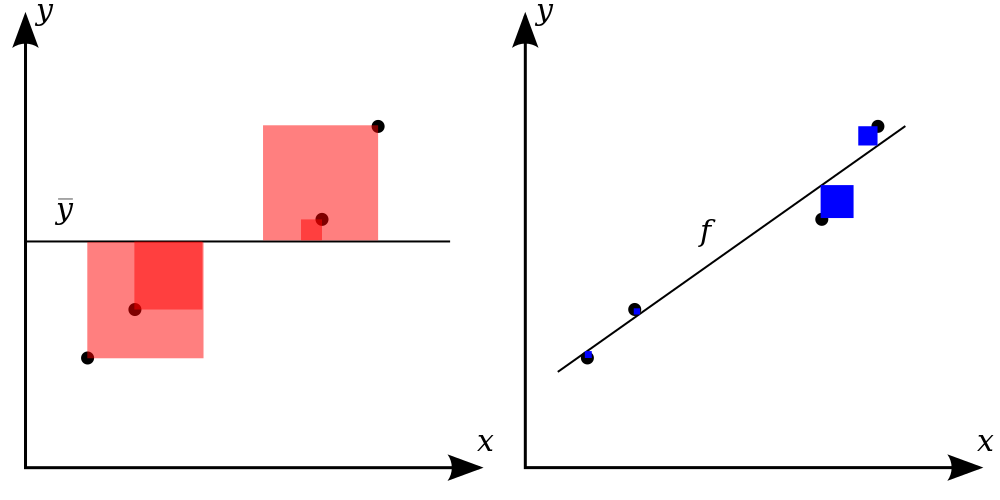
\includegraphics[width=\textwidth]{img/Coefficient_of_Determination.png}
        \caption{Total sum of squares and residual sum of squares}
    \end{figure}
\end{frame}

\section{second section}

\begin{frame}{R2 Score}
    \begin{figure}
        \centering
        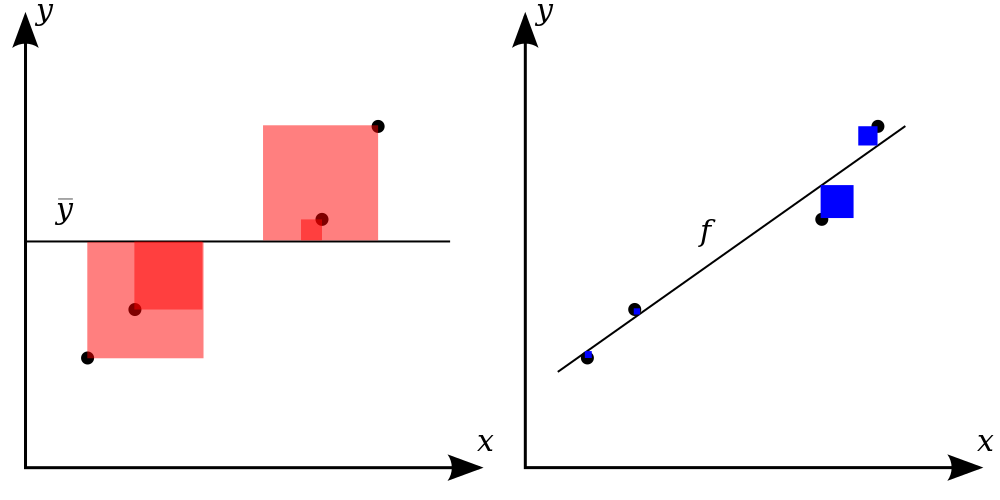
\includegraphics[width=\textwidth]{img/Coefficient_of_Determination.png}
        \caption{Total sum of squares and residual sum of squares}
    \end{figure}
\end{frame}

\end{document}
